% Ubah judul dan label berikut sesuai dengan yang diinginkan.
\section{Tinjauan Pustaka}
\label{sec:tinjauanpustaka}

\subsection{Kursi Roda Elektrik}
Kursi roda adalah perangkat yang dioperasikan secara manual atau digerakkan dengan tenaga yang dirancang terutama untuk digunakan oleh individu dengan disabilitas mobilitas untuk tujuan utama bergerak di dalam ruangan, atau di dalam dan di luar ruangan.  Individu dengan disabilitas mobilitas harus diizinkan menggunakan kursi roda dan alat bantu mobilitas bertenaga manual, misalnya alat bantu jalan, kruk, tongkat, atau perangkat serupa lainnya yang dirancang untuk digunakan oleh individu dengan disabilitas mobilitas, di area mana pun yang terbuka untuk lalu lintas pejalan kaki \cite{ADA_2023}.

%Gambar 2.1
% Contoh input gambar
\begin{figure}[ht]
  \centering

  % Ubah dengan nama file gambar dan ukuran yang akan digunakan
  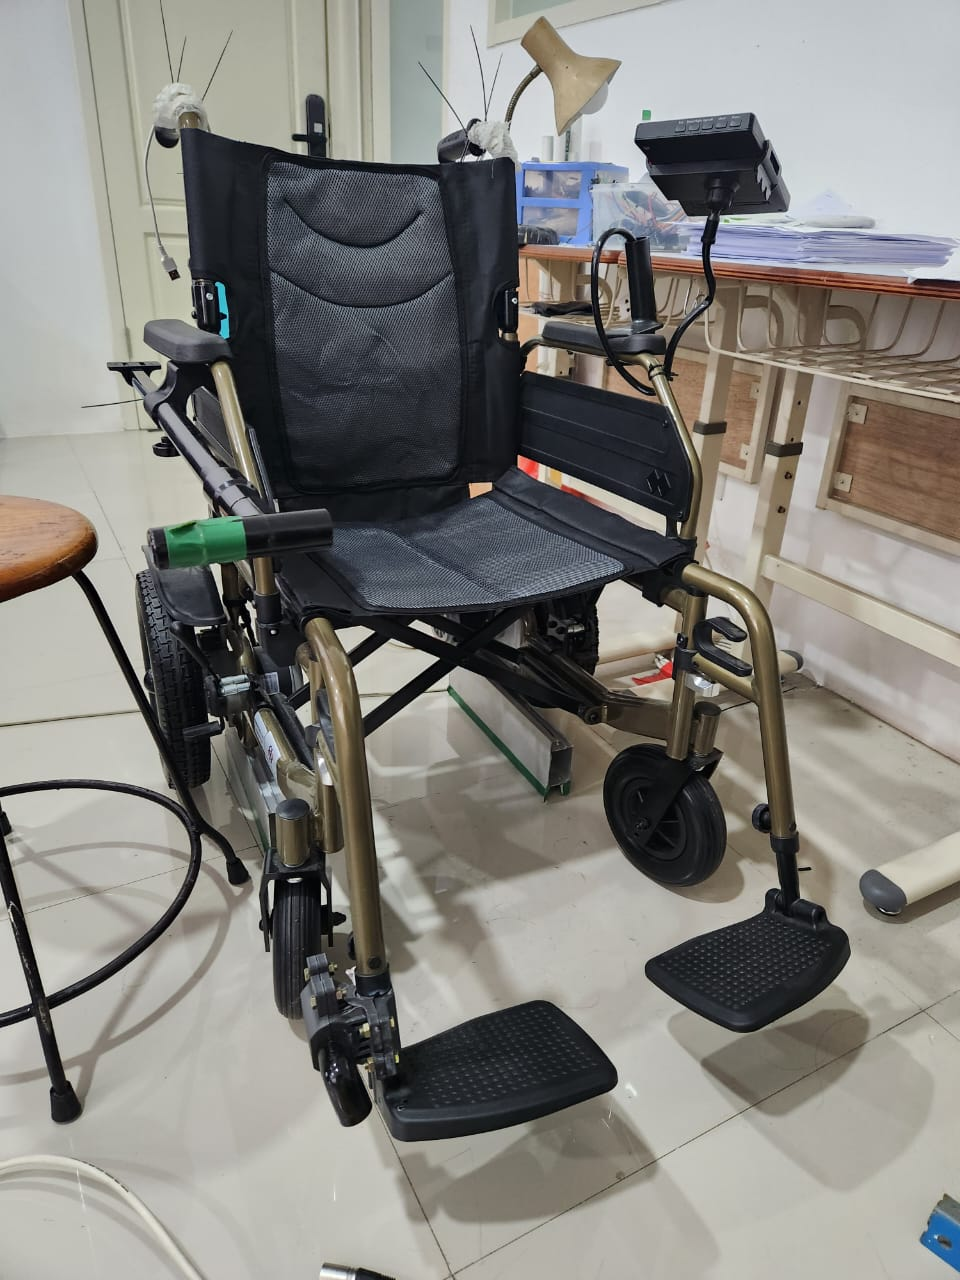
\includegraphics[scale=0.1]{gambar/bab3/kursi.jpeg}

  % Ubah dengan keterangan gambar yang diinginkan
  \caption{Kursi Roda Elektrik}
  \label{fig:kursiroda}
\end{figure}

\subsection{\emph{Eye Gesture}}

\textit{Eye gesture} atau gerakan mata mengacu pada pergerakan mata, seperti tatapan mata, gerakan mata, dan ekspresi wajah, yang memainkan peran penting dalam komunikasi dan interaksi manusia \cite{vanni_2022}. Perangkat pelacak mata telah digunakan untuk mempelajari berbagai aspek gerakan mata, termasuk pengaruh faktor sosial, faktor fisik, dan hubungan antara gerakan mata dan ucapan. Perangkat ini dapat merekam gerakan mata partisipan dengan kamera refleks kornea dan menganalisis gerakan tubuh dan gerakan mata dengan akurasi temporal\cite{gullberg_kita_2009}.

% Gambar 2.2
\begin{figure} [ht] \centering
    % Nama dari file gambar yang diinputkan
    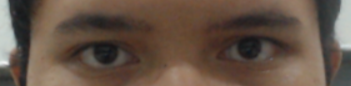
\includegraphics[scale=0.5]{gambar/bab3/gaze.png}
    % Keterangan gambar yang diinputkan
    \caption{Gestur Mata}
    % Label referensi dari gambar yang diinputkan
    \label{fig:gaze}
\end{figure}

\subsection{MediaPipe Face Mesh}

MediaPipe Face Mesh adalah solusi pendeteksi \textit{landmark} wajah yang memperkirakan 468 \textit{landmark} wajah 3D secara real-time, bahkan pada perangkat seluler. Solusi ini menggunakan \textit{pipeline} dari dua jaringan saraf untuk mengidentifikasi koordinat 3D landmark wajah dari gambar 2D. Jaringan pertama, BlazeFace, menghitung lokasi wajah dari gambar penuh, sementara jaringan kedua beroperasi pada wilayah yang dipotong untuk mengidentifikasi lokasi \textit{landmark} \cite{mediapipe_2020}. Teknologi ini memiliki berbagai aplikasi, termasuk deteksi masker wajah, kontrol komputer bebas genggam, dan gerakan yang menyertai ucapan \cite{thaman_2022}.

% Gambar 2.3
\begin{figure} [ht] \centering
    % Nama dari file gambar yang diinputkan
    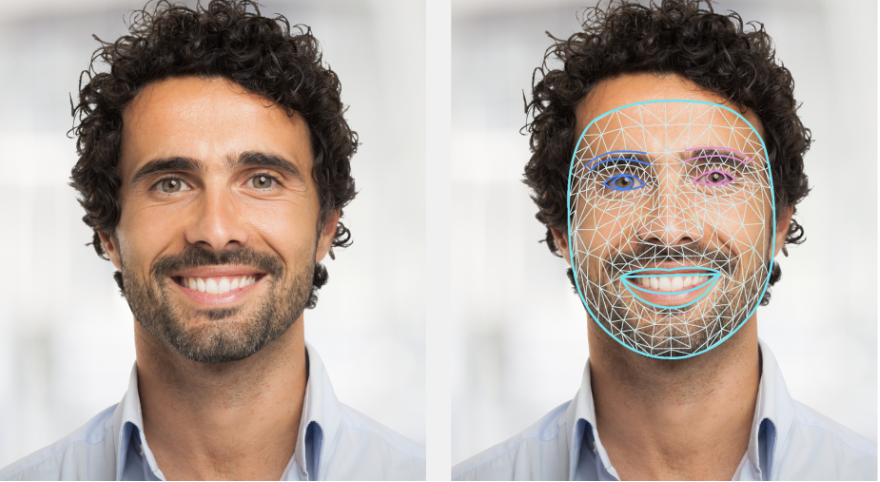
\includegraphics[scale=0.3]{gambar/face_landmark.png}
    % Keterangan gambar yang diinputkan
    \caption{MediaPipe Face Mesh}
    % Label referensi dari gambar yang diinputkan
    \label{fig:facemesh}
\end{figure}

\subsection{\emph{Convolutional Neural Network} (CNN)}

\emph{Convolutional Neural Network} (CNN) adalah jenis jaringan syaraf tiruan yang digunakan terutama untuk pengenalan dan pemrosesan gambar. Ini adalah bagian dari pembelajaran mesin dan dirancang khusus untuk mengidentifikasi dan mengenali objek dalam gambar, serta untuk tugas-tugas seperti klasifikasi objek dan pengenalan pola \cite{arm_2023}. 

Arsitektur pada CNN terdiri dari tiga bagian, yaitu input, \emph{feature learning}, dan \emph{classification}. \emph{Feature Learning} terdiri dari dua buah \emph{convolution layer} dan dua buah \emph{pooling layer}. Pada \emph{classification} terdiri dari dua \emph{hidden layer} dan satu \emph{output layer}. Arsitektur CNN dapat digambarkan seperti pada Gambar \ref{fig:arsitektur cnn}.

% Gambar 2.4
\begin{figure} [ht] \centering
    % Nama dari file gambar yang diinputkan
    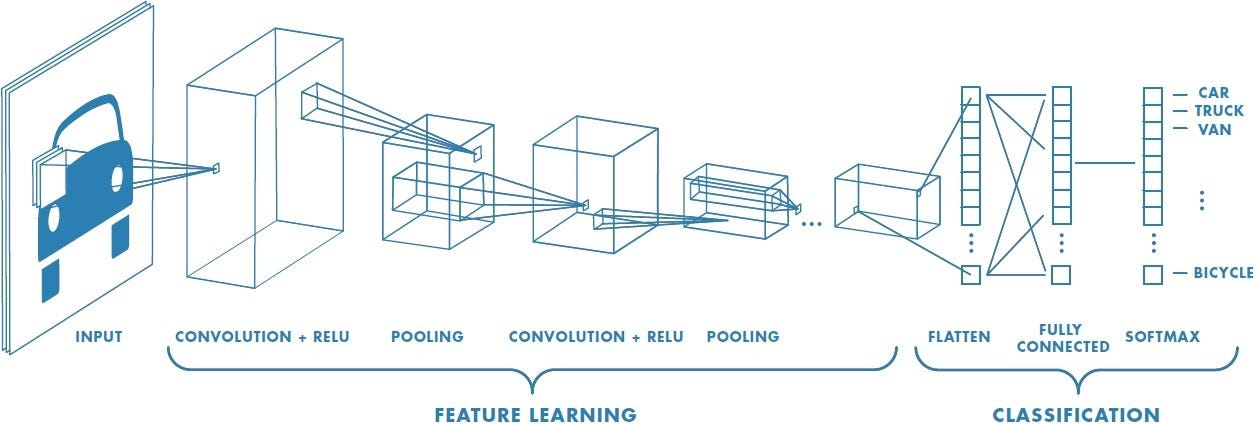
\includegraphics[scale=0.2]{gambar/cnn.jpg}
    % Keterangan gambar yang diinputkan
    \caption{Arsitektur pada \emph{Convolutional Neural Network}}
    % Label referensi dari gambar yang diinputkan
    \label{fig:arsitektur cnn}
\end{figure}

\subsection{\emph{Confusion Matrix}}

\emph{Confusion Matrix} adalah alat yang digunakan untuk mengevaluasi kinerja model klasifikasi dalam pembelajaran mesin. Tabel ini memberikan gambaran mendetail tentang bagaimana model klasifikasi bekerja, menunjukkan hubungan antara prediksi model dengan nilai sebenarnya. \emph{Confusion Matrix} adalah representasi tabel yang terdiri dari empat komponen utama, yaitu \emph{True Positive} (TP), \emph{False Positive} (FP), \emph{True Negative} (TN), dan \emph{False Negative} (FN). Setiap komponen memiliki makna yang spesifik dalam konteks prediksi \cite{provost2013data}. Visualisasi \emph{confusion matrix} dapat dilihat pada Gambar \ref{fig:confusion}.

% Gambar 2.7
\begin{figure} [ht] \centering
    % Nama dari file gambar yang diinputkan
    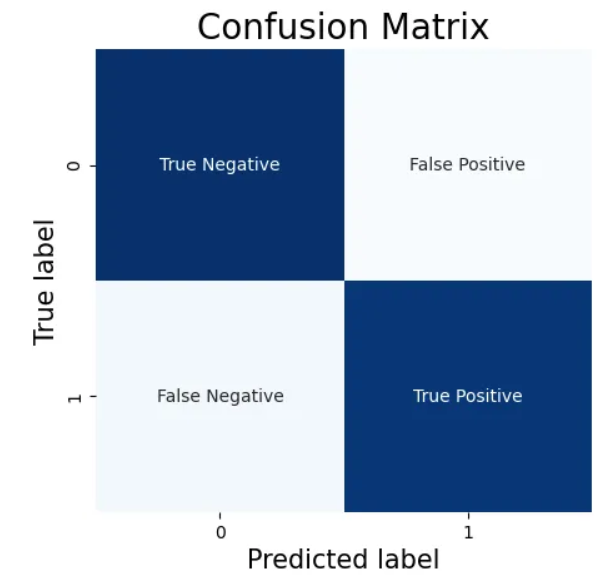
\includegraphics[scale=0.3]{gambar/bab2/confusion.png}
    % Keterangan gambar yang diinputkan
    \caption{Visualisasi \emph{confusion matrix}}
    % Label referensi dari gambar yang diinputkan
    \label{fig:confusion}
\end{figure}

\subsection{\emph{Accuracy}}
\label{subsec:acc_klasifikasi}

\emph{Accuracy} adalah ukuran kinerja yang menunjukkan seberapa tepat model dapat mengklasifikasikan data uji secara benar. Dalam konteks ini, akurasi adalah rasio antara prediksi yang benar (TP dan TN) dengan total jumlah data. Dengan kata lain, akurasi mengukur seberapa dekat nilai prediksi dengan nilai aktual. Nilai \emph{accuracy} dapat diperoleh menggunakan Persamaan \ref{eq:acc}. 

\begin{equation}
  \label{eq:acc}
  Accuracy=\frac{TP+TN}{TP+TN+FP+FN}
\end{equation}

\subsection{\emph{Precision}}
\label{subsec:prec_klasifikasi}

\emph{Precision} adalah ukuran kinerja yang menunjukkan tingkat keakuratan data yang diminta dibandingkan dengan hasil prediksi yang diberikan oleh model. Dalam konteks ini, presisi adalah rasio antara prediksi positif yang benar (TP) dengan total hasil prediksi positif (TP dan FP). Nilai \emph{precision} dapat diperoleh dengan Persamaan \ref{eq:prec}.

\begin{equation}
  \label{eq:prec}
  Precision=\frac{TP}{TP+FP}
\end{equation}

\subsection{\emph{Recall}}
\label{subsec:recall_klasifikasi}

\emph{Recall} adalah ukuran kinerja yang menunjukkan seberapa berhasil model dalam menemukan kembali suatu informasi. Dalam konteks ini, recall adalah rasio antara prediksi positif yang benar (TP) dengan total jumlah data aktual positif (TP dan FN). Dengan demikian, nilai recall dapat dihitung menggunakan Persamaan \ref{eq:recall}.

\begin{equation}
  \label{eq:recall}
  Recall=\frac{TP}{TP+FN}
\end{equation}

\subsection{\emph{F1-Score}}
\label{subsec:score_klasifikasi}

\emph{F1-Score} adalah nilai antara nol (0) hingga satu (1) yang diperoleh dari rata-rata harmonis (\emph{harmonic mean}) antara nilai \emph{precision} dan nilai \emph{recall}. Oleh karena itu, nilai \emph{F1-Score} dapat dihitung menggunakan Persamaan \ref{eq:score}.

\begin{equation}
  \label{eq:score}
  F{1}{-}Score=\frac{2 \times Precision \times Recall}{Precision+Recall}
\end{equation}

\subsection{Implementasi ke Intel NUC}

Implementasi sistem deteksi gerakan mata ke Intel NUC dimulai dengan menginstal pustaka perangkat lunak yang diperlukan, seperti Python, OpenCV, dan Mediapipe, ke dalam perangkat tersebut. Model yang telah dilatih kemudian diintegrasikan dengan program kontrol kursi roda, menghubungkan input dari kamera ke sinyal keluaran untuk motor kursi roda. Intel NUC terhubung ke kamera melalui port USB dan berkomunikasi dengan motor kursi roda melalui protokol serial. Sistem ini dioptimalkan untuk mencapai keseimbangan antara kecepatan dan akurasi, dengan pengaturan parameter model dan komunikasi sehingga memungkinkan kendali kursi roda berbasis gerakan mata yang akurat dan responsif.